\section{Введение}
\subsection{Цель работы}
Цель работы — исследовать зависимость коллекторного тока от напряжения базы в полупроводниковом приборе, вычислить ток насыщения \( I_0 \), а также построить теоретическую кривую зависимости \( I_k = I_0 e^{\frac{e}{kT} U_{\text{эб}}} \) и сравнить её с экспериментальными данными.

\subsection{Решаемые задачи}
\begin{enumerate}
\item Измерить зависимость тока короткого замыкания коллектора биполярного
транзистора от напряжения между эмиттером и базой.
\item По результатам измерений определить отношение заряда электрона к
постоянной Больцмана.
\end{enumerate}

\section{Основная часть}

\subsection{Теоретическая часть}
Ток короткого замыкания $I_k$ в биполярном транзисторе. Пусть \( U_{\text{ЭБ}} \) — напряжение между эмиттером и базой, \( I_0 \) — ток насыщения, \( T \) — температура в кельвинах, \( e \) — заряд электрона, \( k \) — постоянная Больцмана. Тогда ток короткого замыкания \( I_k \) вычисляется по формуле:


\begin{equation}
I_k = I_0 \left( e^{\frac{U_{\text{ЭБ}} e}{kT}} - 1 \right)
\end{equation}


При комнатной температуре единицей можно пренебречь по сравнению с экспонентой, то есть можно считать:
\begin{equation}
I_k = I_0 e^{\frac{U_{\text{ЭБ}} e}{kT}}
\end{equation}

Прологарифмировав, получим:

\begin{equation}
\ln I_k = \ln I_0 + \frac{U_{\text{ЭБ}} e}{kT}
\end{equation}

График \( \ln I_k \) как функции от \( U_{\text{ЭБ}} \) — прямая. Тангенс угла её наклона равен:

\begin{equation}
\tan \alpha = \frac{e}{kT}
\end{equation}

Получаем искомое отношение:

\begin{equation}
T \tan \alpha= \frac{e}{k}
\end{equation}

\begin{equation}
S = \sqrt{\frac{\sum (a_i - \bar{a})^2}{n(n-1)}}
\end{equation}
где \(S\) — стандартная погрешность выборки, \(a_i\) — значения наблюдений, \(\bar{a}\) — среднее значение, \(n\) — количество элементов в выборке.

Измерения проводились дважды с разными шкалами вольтметра.

\subsection{Эксперимент}
На этой схеме:
\begin{itemize}
    \item БП — блок питания электрической схемы;
    \item \( R_1 \) — ограничительный резистор;
    \item \( R_2 \) — потенциометр, с помощью которого можно изменять напряжение \( U_{\text{эб}} \);
    \item \( V_1 \) — вольтметр для измерения \( U_{\text{эб}} \);
    \item \( R_3 \) — резистор в цепи \( к-б \), по падению напряжения на котором можно измерить ток коллектора \( I_{\text{к}} \);
    \item \( V_2 \) — вольтметр для измерения падения напряжения \( U_{\text{кб}} \) на \( R_3 \).
\end{itemize}.

\begin{figure}[ht!]
\centering
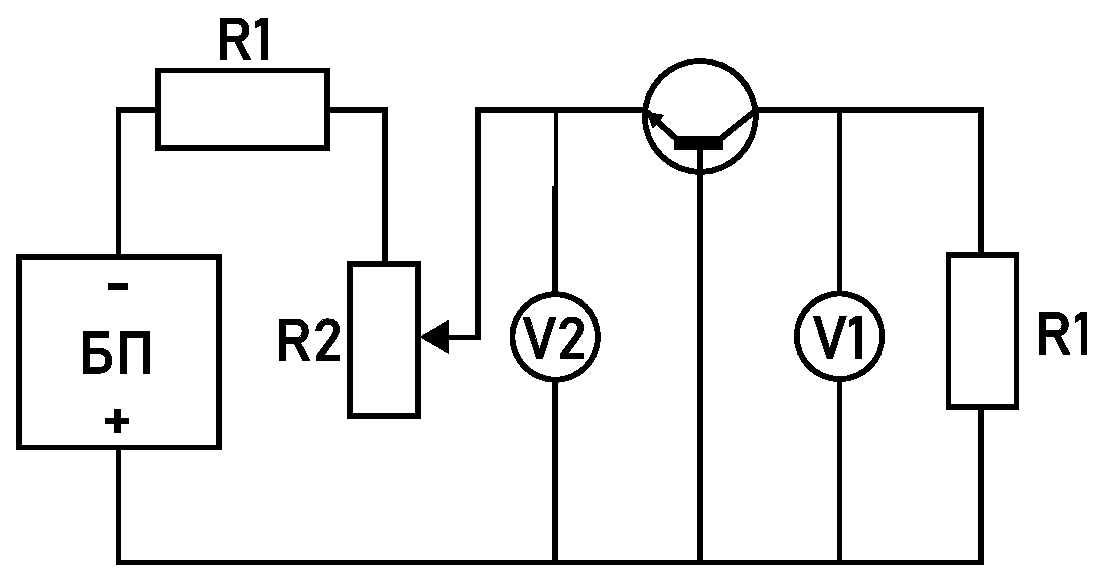
\includegraphics[width=0.9\textwidth]{транзистор.eps}
\caption{Принципиальная электрическая схема установки}
\label{fig:sketch}
\end{figure}

\begin{figure}[H]
\centering
\includegraphics[width=0.6\textwidth]{Установка.jpg}
\caption{Фотография установки -  цифровые
вольтметры, источник электрического питания УПУ-1У4, транзистор П 702А.}
\label{fig:device}
\end{figure}


\subsection{Обработка данных и обсуждение результатов}

\subsubsection{Исходный код}
Для написания программы, вычисляющей все требуемые данные, используется язык C++; среда разработки - Visual Studio.

Программа считывает данные из CSV-файла, выполняет ряд математических операций (вычисление разностей, отношений, среднего, отклонений и стандартной ошибки) и выводит результаты в консоль и записывает в файл CSV. 

\begin{lstlisting}[label=listing1, caption=Функция вычисления среднего]
 double aver(std::vector<double>& a_arr)
{
	double average = 0.0;
	for (int i = 0; i < a_arr.size(); i++)
	{
		average += a_arr[i];
	}
	average /= a_arr.size();

	return average;
}

\end{lstlisting}

Этот код выполняет анализ данных с использованием метода парных точек. Он считывает данные из двух файлов, вычисляет наклон для каждой пары точек, а затем проводит статистический анализ этих наклонов. Для каждой пары точек рассчитываются разницы по координатам \( x \) и \( y \), а затем вычисляется наклон \( a_i\). 

\[
\bar{a} = \frac{1}{N} \sum_{i=1}^{N} a_i
\]
Для расчетов используется t-критическое значение для 95\% доверия:

\[
t_{\text{value}} = 2.3646
\]

\begin{lstlisting}[label=listing2, caption=Функции для расчета отклонений]
std::vector<double> a_arr(std::vector<double>& x_, std::vector<double>& y_)
{
	std::vector<double> a;
	for (int i = 0; i < x_.size(); i++)
	{
		a.push_back(y_[i] / x_[i]);
	}
	return a;
}

std::vector<double> a_diff(std::vector<double>& a, double average)
{
	std::vector<double> arr;
	for (int i = 0; i < a.size(); i++)
	{
		arr.push_back(a[i] - average);
	}
	return arr;
}

std::vector<double> a2_arr(std::vector<double>& arr)
{
	std::vector<double> a;
	for (int i = 0; i < arr.size(); i++)
	{
		a.push_back(arr[i] * arr[i]);
	}
	return a;
}

\end{lstlisting}

\begin{lstlisting}[label=listing3, caption=Функция вычисление стандартной ошибки среднего]
double s(std::vector<double>& a2_arr)
{
	double t = 0.0;
	double sum = 0.0;

	for (int i = 0; i < a2_arr.size(); i++)
	{
		sum += a2_arr[i];
	}

	t = sqrt(sum / (a2_arr.size() * (a2_arr.size() - 1)));

	return t;
}

\end{lstlisting}

\begin{lstlisting}[label=listing4, caption=Код программы реализующим метод парных точек]
	std::vector<double> x_;
	std::vector<double> y_;
	diff(x_, data1);
	diff(y_, data2);

	std::vector<double> a = a_arr(x_, y_);
	double average = aver(a);
	std::vector<double> a_d = a_diff(a, average);
	std::vector<double> a2 = a2_arr(a_d);
\end{lstlisting}

\subsubsection{Таблицы}

\begin{center}
\begin{table}[h!]
\centering
\caption{Грубые измерения}
\label{tabl:3}
\begin{tabular}{|c|c|c|c|c|}
\hline
 №п/п &
\begin{minipage}{2cm}
    $U_{\text{эб}}$
\end{minipage} &
\begin{minipage}{2cm}
    $U_{\text{кб}}$
\end{minipage} &
\begin{minipage}{2cm}
    $I_k = \frac{U_{\text{кб}}}{R_3}$
\end{minipage} &
\begin{minipage}{2cm}
    $\ln I_k$
\end{minipage}\\
\hline
{}&В&В&мА&{}\\
\hline
1 & 0,30 & 0,0014 & 0.117 & -9.056 \\
2 & 0,31 & 0,0021 & 0.175 & -8.650 \\
3 & 0,32 & 0,0041 & 0.342 & -7.981 \\
4 & 0,33 & 0,0075 & 0.625 & -7.377 \\
5 & 0,34 & 0,0133 & 1.108 & -6.804 \\
6 & 0,35 & 0,0178 & 1.483 & -6.513 \\
7 & 0,36 & 0,0297 & 2.475 & -6.001 \\
8 & 0,37 & 0,0400 & 3.333 & -5.704 \\
9 & 0,38 & 0,0588 & 4.9 & -5.319 \\
10 & 0,39 & 0,0727 & 6.058 & -5.106 \\
11 & 0,40 & 0,1085 & 9.042 & -4.706 \\
12 & 0,41 & 0,1301 & 10.841 & -4.524 \\
13 & 0,42 & 0,1602 & 13.35 & -4.316 \\
14 & 0,43 & 0,1809 & 15.075 & -4.195 \\
15 & 0,44 & 0,2123 & 17.691 & -4.035 \\
16 & 0,45 & 0,2430 & 20.25 & -3.900 \\
\hline
\end{tabular}
\end{table}
\end{center}
Среднее значение $\overline{\ln I_k} = -5.887$. 
Среднее значение $\overline{U_{\text{эб}}} = 0.375$. 

\begin{center}
\begin{table}[h!]
\caption{Метод парных точек для грубых измерений}
\begin{tabular}{|c|c|c|c|c|c|c|c|c|c|}

\hline
№ & $x_2$ & $x_1$ & $x_2 - x_1$ & $y_2$ & $y_1$ & $y_2 - y_1$ & $a_i$ & $a_i - a$ & $(a_i - a)^2$ \\
\hline
1 & 0.38 & 0.3 & 0.08 & -5.318 & -9.056 & 3.737 & 46.721 & 12.362 & 152.82 \\ 
2 & 0.39 & 0.31 & 0.08 & -5.106 & -8.651 & 3.544 & 44.305 & 9.946 & 98.926 \\ 
3 & 0.4 & 0.32 & 0.08 & -4.706 & -7.982 & 3.276 & 40.947 & 6.588 & 43.404 \\ 
4 & 0.41 & 0.33 & 0.08 & -4.524 & -7.377 & 2.853 & 35.668 & 1.309 & 1.713 \\ 
5 & 0.42 & 0.34 & 0.08 & -4.316 & -6.805 & 2.489 & 31.108 & -3.251 & 10.566 \\ 
6 & 0.43 & 0.35 & 0.08 & -4.195 & -6.513 & 2.319 & 28.984 & -5.375 & 28.886 \\ 
7 & 0.44 & 0.36 & 0.08 & -4.035 & -6.002 & 1.967 & 24.586 & -9.773 & 95.516 \\ 
8 & 0.45 & 0.37 & 0.08 & -3.899 & -5.704 & 1.804 & 22.552 & -11.806 & 139.396 \\ 

\hline
\end{tabular}
\end{table}
\end{center}


\begin{center}
Среднее значение $a = 34.69$.
\end{center}


Рассчитаем стандартную погрешность выборки по формуле (6):
\begin{center}
$S=3.165$ 1/В
\end{center}

Найдем коэффициент Стьюдента t для 8 элементов и вероятности 0,95 из таблиц: $t = 2.3646$
\[
\tan(\alpha) = 34.69 \pm 7.48 \, \left(\frac{1}{\text{В}}\right)
\]

Определим погрешность измерения искомого отношения как погрешность косвенных измерений по формуле:
\begin{equation}
\Delta \frac{e}{k} = \sqrt{\frac{1}{9} \left( \frac{\partial \frac{e}{k}}{\partial T} \right)^2 \Delta T^2 + \left( \frac{\partial \frac{e}{k}}{\partial \tan \alpha} \right)^2 \Delta \tan \alpha^2 }
\end{equation}
После преобразований получаем следующую формулу:
\begin{equation}
\Delta \frac{e}{k} = \sqrt{\frac{1}{9} \bar{a}^2 \Delta T^2 + T^2 \Delta \tan \alpha^2}
\end{equation}

Где:
\[
\Delta T = 0.5 \, \text{K}, \quad \Delta \tan \alpha = S \cdot t = 7.483 \, \frac{1}{\text{В}}
\]

Тогда для первого измерения:
\[
\frac{e}{k} = (10135.98 \pm 2227.88)~\frac{\text{К}}{\text{В}}
\]

Рассчитываем ток насыщения по формуле:
\begin{equation}
I_0 = \exp\left( \overline{\ln I_k} - \frac{e}{kT} \cdot \overline{U_{\text{эб}}} \right)
\end{equation}


Таким образом, значение тока насыщения равно:
\[
I_0 = 0.7041 \cdot 10^{-8}~\text{мА}
\]

\clearpage

\begin{center}
\begin{table}[h!]
\centering
\caption{Точные измерения}
\label{tabl:3}
\begin{tabular}{|c|c|c|c|c|}
\hline
 №п/п &
\begin{minipage}{2cm}
    $U_{\text{эб}}$
\end{minipage} &
\begin{minipage}{2cm}
    $U_{\text{кб}}$
\end{minipage} &
\begin{minipage}{2cm}
    $I_k = \frac{U_{\text{кб}}}{R_3}$
\end{minipage} &
\begin{minipage}{2cm}
    $\ln I_k$
\end{minipage}\\
\hline
{}&В&В&мА&{}\\
\hline
1& 0.3000&0.0012&0.1&-9.210 \\
2&0.3106&0.0021&0.175&-8.651 \\
3&0.3204&0.0039&0.325&-8.032 \\
4&0.3300&0.0064&0.533&-7.536 \\
5&0.3400&0.0108&0.9&-7.013 \\
6&0.3500&0.0168&1.4&-6.571 \\
7&0.3600&0.0264&2.2&-6.119 \\
8&0.3700&0.0411&3.425&-5.676 \\
9&0.3804&0.0531&4.425&-5.420 \\
10 &0.3900&0.0725&6.042&-5.109 \\
11 &0.4000&0.0937&7.808&-4.852 \\
12 &0.4108&0.1201&10.008&-4.604 \\
13 &0.4202&0.1470&12.25&-4.402 \\
14 &0.4308&0.1810&15.083&-4.194 \\
15& 0.4400&0.2086&17.383&-4.052 \\
16& 0.4500&0.2346&19.55&-3.935 \\
\hline
\end{tabular}
\end{table}
\end{center}
Среднее значение $\overline{\ln I_k} = -5.961$.
Среднее значение $\overline{U_{\text{эб}}} = 0.375$. 
\begin{center}
\begin{table}[h!]
\caption{Метод парных точек для точных измерений}
\begin{tabular}{|c|c|c|c|c|c|c|c|c|c|}

\hline
№ & $x_2$ & $x_1$ & $x_2 - x_1$ & $y_2$ & $y_1$ & $y_2 - y_1$ & $a_i$ & $a_i - a$ & $(a_i - a)^2$ \\
\hline
1 & 0.3804 & 0.3000 & 0.0804 & -5.420 & -9.210 & 3.789 & 47.137 & 12.443 & 154.83 \\ 
2 & 0.3900 & 0.3106 & 0.0794 & -5.109 & -8.651 & 3.541 & 44.605 & 9.910 & 98.222 \\ 
3 & 0.4000 & 0.3204 & 0.0796 & -4.852 & -8.031 & 3.179 & 39.938 & 5.244 & 27.504 \\ 
4 & 0.4108 & 0.3300 & 0.0808 & -4.604 & -7.536 & 2.932 & 36.287 & 1.593 & 2.537 \\ 
5 & 0.4202 & 0.3400 & 0.0802 & -4.402 & -7.013 & 2.610 & 32.554 & -2.139 & 4.578 \\ 
6 & 0.4308 & 0.3500 & 0.0808 & -4.194 & -6.571 & 2.377 & 29.419 & -5.274 & 27.820 \\ 
7 & 0.4400 & 0.3600 & 0.08 & -4.052 & -6.119 & 2.067 & 25.838 & -8.856 & 78.430 \\ 
8 & 0.4500 & 0.3700 & 0.08 & -3.934 & -5.676 & 1.741 & 21.773 & -12.921 & 166.952 \\ 


\hline
\end{tabular}
\end{table}
\end{center}

Аналогично получаем следующие значения: 
\begin{enumerate}
    \item$S=3.165$ 1/В;
    \itemСреднее $a=34.69$;
    \item$\tan(\alpha) = 34.69 \pm 7,48 \, \left(\frac{1}{\text{В}}\right)$;
    \item$\frac{e}{k} = (10234.8 \pm 2207.6)~\frac{\text{К}}{\text{В}}$;
\end{enumerate}
Ток насыщения:
\[
I_0 = 0.57 \cdot 10^{-8}~\text{мА}
\]

\subsubsection{Графики}



\begin{figure}[ht!]
\centering
\includegraphics[width=0.9\textwidth]{diode_ln_curve.eps}
\caption{Зависимость $\ln I_k$ от $U_{\text{эб}}$ на грубой шкале}
\label{fig:plot}
\end{figure}

\begin{figure}[ht!]
\centering
\includegraphics[width=0.9\textwidth]{diode_curve.eps}
\caption{Зависимость тока коллектора от напряжения эмиттер-база на грубой шкале}
\label{fig:plot}
\end{figure}

\begin{figure}[ht!]
\centering
\includegraphics[width=0.9\textwidth]{diode_ln_curve1.eps}
\caption{Зависимость $\ln I_k$ от $U_{\text{эб}}$ на точной шкале}
\label{fig:plot}
\end{figure}

\begin{figure}[ht!]
\centering
\includegraphics[width=0.9\textwidth]{diode_curve1.eps}
\caption{Зависимость тока коллектора от напряжения эмиттер-база на точной шкале}
\label{fig:plot}
\end{figure}
\clearpage
\section{Вывод}
 Экспериментально определено отношение элементарного заряда к постоянной Больцмана посредством анализа зависимости тока короткого замыкания коллектора биполярного транзистора от напряжения между эмиттером и базой. Для визуализации зависимости построены графики. Погрешность определения искомой величины оценена как погрешность косвенных измерений.
% Список литературы
% Для отчёта он не обязателен
\begin{thebibliography}{9}

%ссылка на репозиторий с исходныим кодом отчета и всех расчетных программ обязательна 
\bibitem{repo}
\url{https://github.com/st117210/Workshop4.git}  

\end{thebibliography}
\clearpage
\appendix